\section{Aufbau}
\label{sec:Aufbau}
Im Bild \ref{fig:Versuchsaufbau} ist der Versuchsaufbau zu sehen. Der Rezipient (R) ist mit der Turbomolekularpumpe (P2) verbunden, 
welche wiederum mit der Drehschieberpumpe (P1) verbunden ist. Über das Ventil (V1) kann die Drehschieberpumpe vom 
restlichen Aufbau abgeschiebert werden. Dasselbe ist für die Turbopumpe mit dem Ventil (V2) möglich.
Zum Belüften des Rezipienten sind ein Ventil (V3) und ein Drosselventil (D1) mit dem Rezipienten verbunden.
Die für den Versuch genutzten Messgeräte sind zum einen das Pirani-Kaltkathoden-Vakuummeter (M1) zur Bestimmung der 
von der Turbopumpe erzeugten Drücke und das Piezo-Pirani-Vakuummeter (M2) für die Drücke, die durch die Drehschieberpumpe 
erzeugt werden.

    \begin{figure}
        \centering
        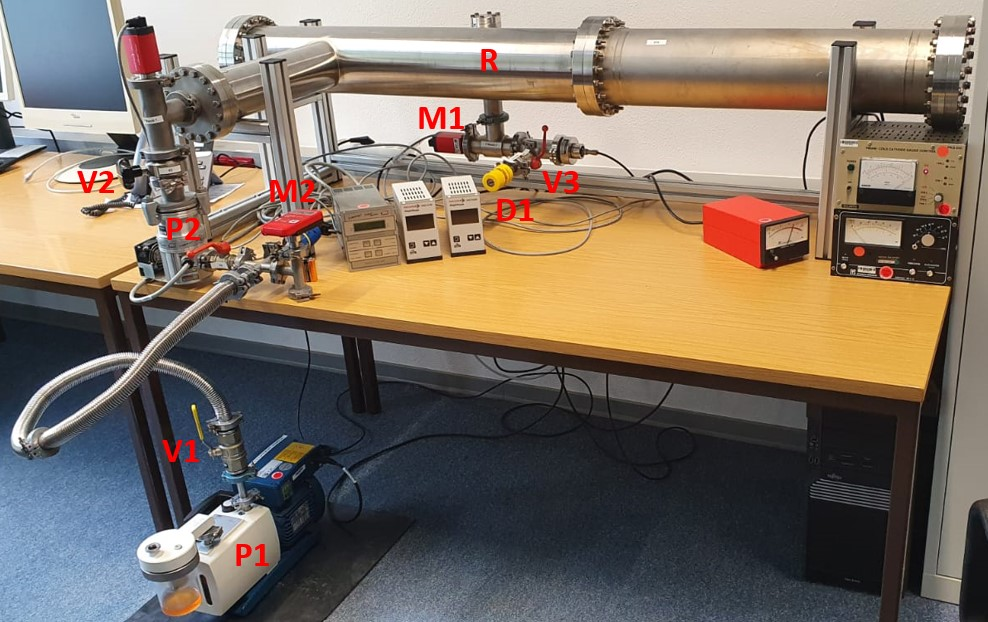
\includegraphics[width=1\textwidth]{Versuchsaufbau_V70.jpeg}
        \caption{Versuchsaufbau.}
        \label{fig:Versuchsaufbau}
    \end{figure}


\section{Durchführung}
\label{sec:Durchführung}
Bevor die eigentlichen Messungen beginnen können, muss überprüft werden ob der Rezipient dicht ist.
Dafür wird der Rezipient evakuiert und festgestellt ob der Enddruck im Bereich des von der angeschlossenen Pumpe, maximal erzeugbaren Vakuums liegt. 
Ist dies nicht der Fall, muss die Apparatur mit z.b. Blindflanschen, durch Ventile schließen oder Umbaumaßnahmen überprüft werden und undichte Stellen abgedichtet werden.

\subsection{Messung mit der Turbomolekularpumpen}
\label{sec:Turbomolekularpumpen Messungen}
Da die Turbomolekularpumpe schon vor Beginn des Versuchs lief, wurde mit der Bestimmung des Saugvermögens der Turbopumpe begonnen.

\subsubsection{Evakuierungskurve}
\label{sec:Evakuierungskurve1}
Zur Bestimmung der Evakuierungskurve laufen beide Pumpen und die Ventile zum Rezipienten sind geöffnet.
Nun wird der Rezipient vorsichtig mit geöffnetem V3 und über das Drosselventil (D1) belüftet, bis der Druck im Rezipienten bei $p_0 = 5 \cdot 10^{-3}$ liegt.
Anschließend wird V3 geschlossen und für 120 s alle 10 s der Druck im Rezipienten abgelesen.
Diese Prozedur wird 3-mal durchgeführt.

\subsubsection{Leckratenmessung}
\label{sec:Leckratenmessung1}
Für die Leckratenmessung wird bei laufenden Pumpen und geöffneten V1 und V2 über das Drosselventil ein Gleichgewichtsdruck eingestellt.
Danach wird die Turbomolekularpumpe durch Schließen des Ventils V2 abgeschiebert und 120 s lang alle 10s der Druck gemessen.
Dies wird insgesammt 3-mal pro Gleichgewichtsdruck und mit vier verschiedenen Gleichgewichtsdrücken ($p_g = 5 \cdot 10^{-5}; 7 \cdot 10^{-5}; 1 \cdot 10^{-4}; 2 \cdot 10^{-4}$ mbar) durchgeführt.

\subsection{Messung mit der Drehschieberpumpen}
\label{sec:Drehschieberpumpen Messungen}
Für die Messungen mit der Drehschieberpumpe wird die Turbomolekularpumpe ausgestellt. Das Ventil V2 bleibt die gesamte Zeit geöffnet.

\subsubsection{Evakuierungskurve}
\label{sec:Evakuierungskurve2}
Bei der Bestimmung der Evakuierungskurve der Drehschieberpumpe bleiben V1 und V2 geöffnet, der Rezipient wird über V3 und D1 geflutet, 
bis Atmosphärendruck innerhalb des Rezipienten herrscht. Dann wird V3 geschlossen und 600 s lang alle 10 s der Druck im Rezipienten abgelesen.
Auch diese Messung wir 3-mal durchgeführt.

\subsubsection{Leckratenmessung}
\label{sec:Leckratenmessung2}
Die Leckratenmessung der Drehschieberpumpe verläuft fast äquivalent zur Messung mit der Turbomolekularpumpe.
Über das Drosselventil D1 werden vier verschiedene Gleichgewichtsdrücke ($p_g = 0,5; 10; 50; 100\: mbar$) eingestellt.
Anschließend wird die Pumpe über V1 abgeschiebert und 200 s alle 10 s der Druck bestimmt. Für jeden Gleichgewichtsdruck 
wird die Messung wieder 3-mal durchgeführt.


